\chapter{Problemanalyse und Anforderungsdefinition}
\label{cha:pua}

\emph{» Das Spiel ist die höchste Form der Forschung. «} \\
(Albert Einstein) \\

In Abschnitt \ref{sec:Die Problematik} wird die Aufgabenstellung genauer analysiert, die Spieltheoretischen Verfahren und die Verfahren des maschinellen Lernens aus dem Grundlagenkapitel werden auf die beiden Strategiespiele Reversi und Tic Tic Toe angewendet. Abschnitt \ref{sec:Anforderungen} definiert die Anforderungen die der Softwareprototyp erfüllen sollte. Die Anforderungen beziehen sich auf die Problematik und die Grundlagen. 

\section{Die Problematik}
\label{sec:Die Problematik}
Das Thema der Arbeit ist Untersuchung der Lernfähigkeit verschiedener Verfahren am Beispiel von Computerspielen. Bevor die Lernfähigkeit der Verfahren untersucht werden kann, müssen wir die Computerspiele festlegen und analysieren. Wie bereits erwähnt werden wir die Lernfähigkeit der Verfahren am Beispiel der Strategiespiele Reversi und Tic Tac Toe untersuchen (siehe Abbildung \ref{fig:reversi_und_tictactoe}). Eine genaue Beschreibung der Spielregeln, der Siegesbedingungen und möglicher Strategien bezüglich Heuristiken, wird in Kapitel \ref{cha:Modellierung und Entwurf} Modellierung und Entwurf erfolgen. Die zentrale Frage ist: wie kann ein Programm lernen ein Computerspiel erfolgreich zu spielen? \\

\begin{figure}[!htbp]
  \centering
  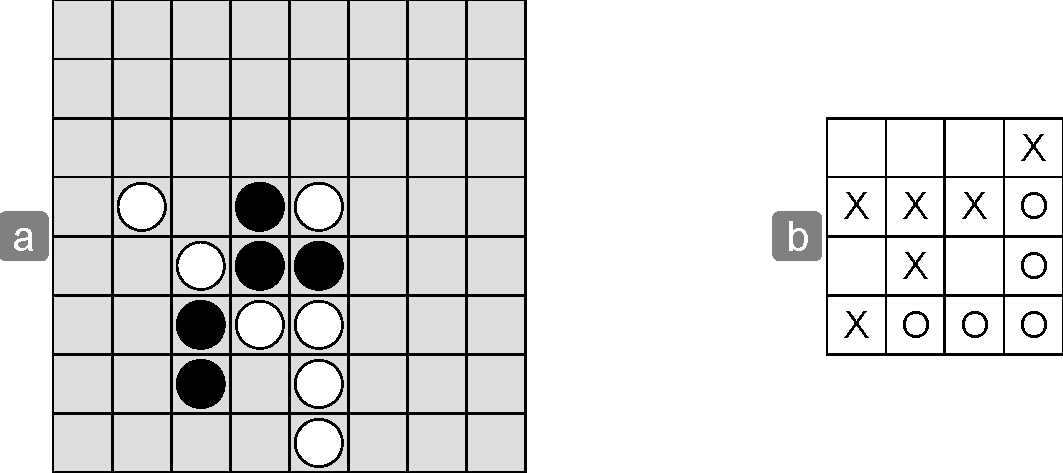
\includegraphics[scale = 0.8]{inhalt/abbildungen/reversi_und_tictactoe.pdf}
  \caption{Tic Tac Toe und Reversi Spielzustände.}
  \label{fig:reversi_und_tictactoe}
\end{figure} 

\paragraph{Die Spieltheorie} aus Abschnitt \ref{sec:Spiele mit Gegner} liefert gleich mehrere Ansätze diese Frage zu beantworten. Die kombinatorische Suche (Abschnitt \ref{subsec:Minimax} Minimax) probiert einfach alle Möglichkeiten aus und liefert die beste gefundene Möglichkeit zurück. Die reine kombinatorische Minimax Suche ist praktisch jedoch nicht anwendbar, da, wie bereits im Abschnitt Minimax beschrieben wurde, die Anzahl der Kombinationsmöglichkeiten mit der Komplexität des Ausgangsproblems exponentiell ansteigt. \\

Selbst mit einer Kürzung von ganzen Unterbäumen des Suchbaums, ist die Rechenzeit für realistische Probleme nicht handhabbar (siehe Abschnitt \ref{subsec:Alpha-Beta-Kürzung} Alpha-Beta-Kürzung). Das Kürzen des Suchbaums kann unter Umständen mit einer iterativ vertiefenden Tiefensuche verbessert werden (siehe Abschnitt \ref{subsec:Iterativ vertiefende Tiefensuche} Iterativ vertiefende Tiefensuche). Die iterativ vertiefende Suche könnte Züge, z.B. in einer Tiefe von 2, sortieren. Vielversprechende Spielzüge könnten zu erst ausprobiert werden und das Alpha-Beta Verfahren könnte einen größeren Teil des Suchbaums kürzen. \\

Eine weitere Möglichkeit die Suche nach dem optimalen Spielzug in jeder Spielsituation zu verbessern, ist das Vermeiden von Übergängen. Ein Übergang oder Transition ist ein Spielzustand der mehrfach, an verschiedenen Stellen, in einem Suchbaum auftreten kann. Übergangstabellen und Transitions sind ausführlich in Abschnitt \ref{subsec:Übergangstabellen} Übergangstabellen erläutert. Eine Vermeidung dieser Übergänge könnte eine weitere Rechenzeitverringerung bewirken. \\

Die Heuristik oder Bewertungsfunktion ist wohl der wichtigste Leistungsfaktor aus den Verfahren der Spieltheorie (siehe Abschnitt \ref{subsec:Heuristik} Heuristik). Eine Heuristik kann jeden Knoten des Suchbaums bewerten (Nutzwert) und nicht nur die Blätter. Dies ermöglicht es die Suche nach einer bestimmten Zeitspanne oder iterierten Tiefe abzubrechen und den Spielzustand mit der besten Bewertung zurück zu geben. \\

Die Vorteile einer Heuristik sind die Limitierung der Zeit, die für eine Suche benötigt wird und dass das bisher beste gefundene Ergebnis zurück gegeben wird. Der große Nachteil einer Bewertungsfunktion ist, ein ermittelter Nutzwert für einen Spielzustand kann falsch sein. Die Qualität einer Heuristik ist also ausschlaggebend für die Spielstärke des Programms. Heuristiken sind zudem stark abhängig von ihrer Spielgrundlage, d.h. sowohl Reversi als auch Tic Tac Toe benötigen eigene Heuristiken, die individuell den Nutzen der Stellungen bewerten. \\

\begin{figure}[!htbp]
  \centering
  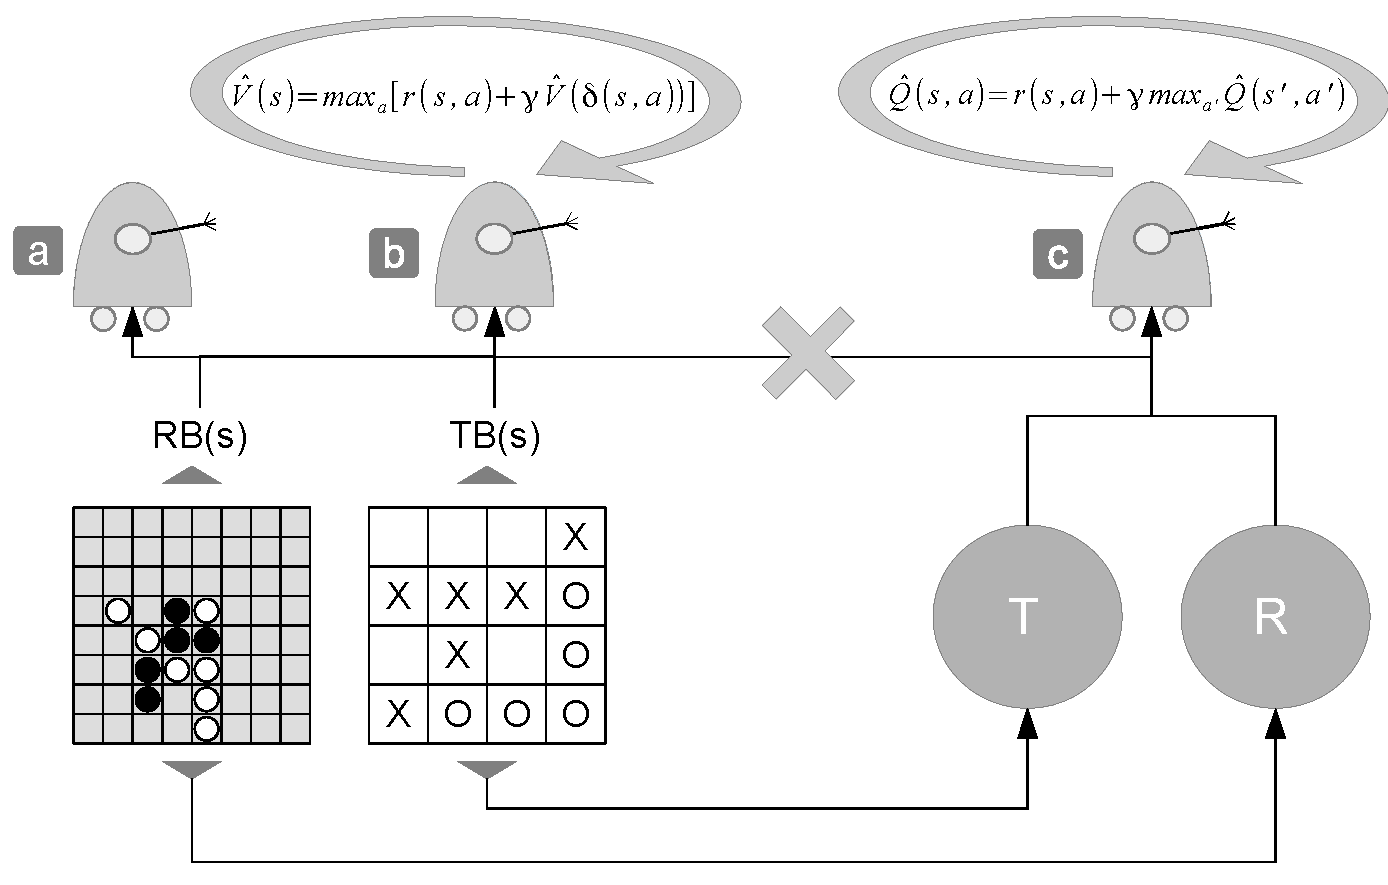
\includegraphics[scale = 0.6]{inhalt/abbildungen/drei_agenten.pdf}
  \caption{Die Projektproblematik.}
  \label{fig:drei_agenten}
\end{figure} 

\paragraph{Die drei Agenten} aus Abbildung \ref{fig:drei_agenten} repräsentieren drei Programme, die mit unterschiedlichen Verfahren, die selbe Aufgabe lösen. Die Aufgabe lautet: für jeden Spielzustand der Strategiespiele Reversi und Tic Tac Toe sollen die Agenten (a), (b) und (c) einen optimalen Spielzug (eine Aktion) vorschlagen, d.h. die Agenten müssen eine optimale Strategie anwenden. Eine optimale Strategie verwendet für jeden Möglichen Spielzustand immer den bestmöglichen Spielzug. \\

Agent (a) ist ein nicht lernender Agent, der Verfahren aus der Spieltheorie anwendet und dem die Bewertungsfunkionen RB(s) und TB(s) zur Verfügung stehen. RB(s) ist die Reversi Bewertungsfunktion, mit einem Reversi Spielzustand s als Eingabeparameter. TB(s) ist die Tic Tac Toe Bewertungsfunktion, mit einem Tic Tac Toe Spielzustand s als Eingabeparameter. \\

Agent (b) ist ein lernender Agent, der wie der Agenten (a) über die Bewertungsfunktionen RB(s) und TB(s) verfügt. Dieser Agent soll die Gewichtungen (Faktoren $a_x$) der Bewertungsfunktionen mittels Spielerfahrung lernen. Er spielt eine festgelegte Anzahl von Spielen z.B. gegen sich selbst und verwendet eine Aktualisierungsfunktion $\hat{V}(s,a)$. Diese Funktion wurde bereits in Abschnitt \ref{subsec:Wert-Iteration und Dynamische Programmierung} Wert-Iteration und Dynamische Programmierung behandelt. Zusammengefasst ist diese Funktion eine Iterationsvorschrift, die mit der Bellman-Rekursionsgleichung die Gewichtungen der Heuristik so lange anpasst, bis diese sich nicht weiter verändern lassen und gegen eine optimale Strategie konvergieren. \\

Agent (c) ist ein lernender Agent, der im Gegensatz zu den Agenten (a) und (b) über kein Modell der Spielwelt verfügt, also ist ihm nicht bekannt in welchen Spielzustand ihn seine Aktionen führen. Er erhält auch keine Bewertungsfunktionen RB(s) und TB(s) für Spielzustände s. Alles was der Agent erhält sind zwei Menge T und R. Menge T enthält alle möglichen Aktionen die der Agent in einer bestimmten Tic Tac Toe Spielsituation ausführen darf, äquivalent dazu enthält Menge R alle möglichen Aktionen die der Agent in einer bestimmten Reversi Spielsituation ausführen darf. Nach einer bestimmten Anzahl von Aktionen erhält der Agent verspätet unterschiedliche Belohnungen für einen Sieg, eine Niederlage oder ein Unentschieden des Spiels. Der Agent verwendet das Lernverfahren $\hat{Q}$(s, a) aus Abschnitt  \ref{subsec:Q-Lernen}, um eine optimale Strategie zu lernen. \\

Sind alle Agenten implementiert, können wir beginnen die Lernfähigkeit der Agenten zu vergleichen. Wie werden die beiden lernenden Agenten gegen den nicht lernenden Agenten abschneiden? Welcher Agent wird der, der am meisten gewinnt und welcher Agent wird am meisten Verlieren? Wie viel Zeit benötigen die Agenten für die Berechnung der optimalen Strategie für die beiden Strategiespiele (Training)? Diese Fragen werden in Kapitel \ref{Auswertung} Auswertung beantwortet.

\section{Anforderungen}
\label{sec:Anforderungen}
Im nachfolgenden Abschnitt definieren wir die funktionalen Anforderungen der Software. Wir bestimmten, welche Funktionalitäten die Strategiespiele und die Agenten mindestens haben und wie die Agenten getestet werden sollen. Wir definieren die Funktionalitäten, um den Funktionsbereich der Software einzugrenzen und einen Überblick zu verschaffen.

\subsection{Tic Tac Toe Spielumgebung}
Die Spielumgebung soll die in Abschnitt \ref{sec:Das Strategiespiel Tic Tac Toe} definierten Tic Tac Toe Spielregeln implementieren. Die Tic Tac Toe Spielumgebung repräsentiert eine Testumgebung für die Agenten, der Zufallsagent wird in dieser Umgebung gegen den TicTacToe-Heuristik Agenten antreten. Der TD-Q-Lernende Agent soll zuerst diese Umgebung erkunden und lernen sich in der Umgebung zurecht zu finden, d.h. der TD-Q-Lernende Agent soll eine TicTacToe-Siegesstrategie entwickeln. 

\myparagraph{makeMove(position):}
Die Funktion soll Koordinaten erhalten. Die Koordinaten definiert exakt, auf welches Spielfeld eine Spielfigur gesetzt werden soll. Die Funktion soll diesen Spielzug, sollte dieser Regelkonform sein, ausführen.

\myparagraph{undoMove():}
Die Funktion soll den letzten durchgeführten Spielzug revidieren.

\myparagraph{getPossibleMoves(): return list}
Die Funktion soll eine Liste von Koordinaten liefern. In dieser Liste sind nur mögliche und regelkonforme Spielzüge (Koordinaten) enthalten.

\myparagraph{isTerminal: return bool}
Die Funktion soll True zurück liefern, wenn der aktuelle Zustand der Umgebung ein Endzustand (Terminalzustand) ist, andernfalls liefert die Funktion ein False.

\myparagraph{getReward: return float}
Die Funktion soll eine nummerische Belohnung liefern. Die Belohnung soll abhängig sein vom aktuellen Spielzustand.

\subsection{Reversi Spielumgebung}
Die Spielumgebung soll die in Abschnitt \ref{sec:Das Strategiespiel Reversi} definierten Reversi Spielregeln implementieren. Die Reversi Spielumgebung repräsentiert eine Testumgebung für die Agenten, der Zufallsagent wird in dieser Umgebung gegen den Reversi-Heuristik Agenten antreten. Der TD-Q-Lernende Agent soll zuerst diese Umgebung erkunden und lernen sich in der Umgebung zurecht zu finden, d.h. der TD-Q-Lernende Agent soll eine Reversi-Siegesstrategie entwickeln. 

\myparagraph{makeMove(position):}
Die Funktion soll Koordinaten erhalten. Die Koordinaten definiert exakt, auf welches Spielfeld eine Spielfigur gesetzt werden soll. Die Funktion soll diesen Spielzug, sollte dieser Regelkonform sein, ausführen.

\myparagraph{undoMove():}
Die Funktion soll den letzten durchgeführten Spielzug revidieren.

\myparagraph{getPossibleMoves(): return list}
Die Funktion soll eine Liste von Koordinaten liefern. In dieser Liste sind nur mögliche und regelkonforme Spielzüge (Koordinaten) enthalten.

\myparagraph{isTerminal: return bool}
Die Funktion soll True zurück liefern, wenn der aktuelle Zustand der Umgebung ein Endzustand (Terminalzustand) ist, andernfalls liefert die Funktion ein False.

\myparagraph{getReward: return float}
Die Funktion soll eine nummerische Belohnung liefern. Die Belohnung soll abhängig sein vom aktuellen Spielzustand.

\subsection{Agent des Zufalls}
Der Agent des Zufalls soll den schlechtesten Spieler symbolisieren. Er soll seine Entscheidungen vollkommen zufällig treffen. In Kapitel \ref{cha:Validierung} Validierung werden wir diesen Agenten, als Gegenspieler für die Heuristik Agenten und die lernenden TD-Q-Agenten einsetzen. \\

\myparagraph{suggestRandomTicTacToeAction(ticTacToeState): return tuple}
Diese Funktion soll eine Tic Tac Toe Spielsituation übergeben bekommen, d.h. eine Instanz der TicTacToe Klasse. Die Funktion soll eine zufällige, aber zulässige, Aktion zurückgeben.

\myparagraph{suggestRandomReversiAction(reversiState): return tuple}
Diese Funktion soll eine Reversi Spielsituation übergeben bekommen, d.h. eine Instanz der Reversi Klasse. Die Funktion soll eine zufällige, aber zulässige, Aktion zurückgeben.

\subsection{Tic Tac Toe Heuristik Agent}
Der Agent soll die in Abschnitt \ref{subsec:Heuristik} erstellte Tic Tac Toe Heuristik und eine 2-Spielzüge vorausschauende Alpha-Beta Suche verwenden (siehe Abschnitt \ref{subsec:Iterativ vertiefende Tiefensuche} und \ref{subsec:Alpha-Beta-Kürzung}). Dieser Agent soll einen fortgeschrittenen Spielgegner repräsentiert, d.h. wir müssen mittels Testspielen gegen den Zufallsagenten zeigen, dass der Tic Tac Toe Heuristik Agent verhältnismäßig oft gewinnt. Dieser Agent soll in Tic Tac Toe Testspielen gegen den TD-Q-Agenten antreten. Die Ergebnisse sollen dabei helfen, die Leistungsfähigkeit und Grenzen des TD-Q-Lernens, hinsichtlich dem Lernen von Tic Tac Toe, zu beurteilen. 

\myparagraph{suggestAction(ticTacToeState): return tuple}
Diese Funktion soll eine Tic Tac Toe Spielsituation übergeben bekommen. Die Funktion soll, abhängig von der erhaltenen Spielsituation, eine Aktion vorschlagen. Die Aktion soll mittels der TicTacToe-Heuristik und eienr 2-Zug Vorausschau und Alpha-Beta-Suche ermittelt werden.

\subsection{Reversi Heuristik Agent}
Der Agent soll die in Abschnitt \ref{subsec:Heuristik} erstellte Reversi Heuristik und eine 2-Spielzüge vorausschauende Alpha-Beta Suche verwenden (siehe Abschnitt \ref{subsec:Iterativ vertiefende Tiefensuche} und \ref{subsec:Alpha-Beta-Kürzung}). Dieser Agent soll einen fortgeschrittenen Spielgegner repräsentiert, d.h. wir müssen mittels Testspielen gegen den Zufallsagenten zeigen, dass der Reversi-Heuristik Agent verhältnismäßig oft gewinnt. Dieser Agent soll in Reversi Testspielen gegen den TD-Q-Agenten antreten. Die Ergebnisse sollen dabei helfen, die Leistungsfähigkeit und Grenzen des TD-Q-Lernens, hinsichtlich dem Lernen von Reversi, zu beurteilen.

\myparagraph{suggestAction(reversiState): return tuple}
Diese Funktion soll eine Reversi Spielsituation übergeben bekommen. Die Funktion soll, abhängig von der erhaltenen Spielsituation, eine Aktion vorschlagen. Die Aktion soll mittels der Reversi Heuristik und eienr 2-Zug Vorausschau und Alpha-Beta-Suche ermittelt werden.

\subsection{Tic Tac Toe TD-Q lernender Agent}
Der Agent soll, mittels des in Abschnitt \ref{sec:TD-Q-Lernen} behandelten TD-Q-Lernens, eine Siegesstrategie für das Strategiespiel Tic Tac Toe entwickeln. Testspiele gegen den Zufallsagenten und den Tic Tac Toe Heuristik Agenten, sollen eine Untersuchung der Leistungsfähigkeit und der Grenzen des TD-Q-Lernens ermöglichen.

\myparagraph{learnTicTacToeInXGames(amountOfGames):}
Die Funktion soll den Lernmodus des Agenten realisieren. Der Eingabeparameter legt die Anzahl der Trainingsspiele fest. Die Lernerfahrungen während dieser Trainingsspiele, sollen in einer SQLite Datenbank gespeichert werden.

\myparagraph{suggestAction(ticTacToeState): return tuple}
Die Funktion soll eine Tic Tac Toe Spielsituation übergeben bekommen. Ausgehend von der Eingangsspielsituation, ist nur eine bestimmte Anzahl von Aktionen möglich. Abhängig von seinen Erfahrungen und dem gegebenen Spielzustand, soll der Agent die mögliche Aktion mit dem höchsten gelernten Q-Wert zurückgeben.

\subsection{Reversi TD-Q lernender Agent}
Der Agent soll, mittels des in Abschnitt \ref{sec:TD-Q-Lernen} behandelten TD-Q-Lernens, eine Siegesstrategie für das Strategiespiel Reversi entwickeln. Testspiele gegen den Zufallsagenten und den Reversi Heuristik Agenten, sollen eine Untersuchung der Leistungsfähigkeit und der Grenzen des TD-Q-Lernens ermöglichen.

\myparagraph{learnReversiInXGames(amountOfGames):}
Die Funktion soll den Lernmodus des Agenten realisieren. Der Eingabeparameter legt die Anzahl der Trainingsspiele fest. Die Lernerfahrungen während dieser Trainingsspiele, sollen in einer SQLite Datenbank gespeichert werden.

\myparagraph{suggestAction(reversiState): return tuple}
Die Funktion soll eine Reversi Spielsituation übergeben bekommen. Ausgehend von der Eingangsspielsituation, ist nur eine bestimmte Anzahl von Aktionen möglich. Abhängig von seinen Erfahrungen und dem gegebenen Spielzustand, soll der Agent die mögliche Aktion mit dem höchsten gelernten Q-Wert zurückgeben.

\subsection{Testen der Agenten}
Eine Testumgebung, in der alle Agenten gegeneinander Spielen. Der Zufallsagent soll in 100 Testspielen gegen den Tic Tac Toe Heuristik Agenten, den Reversi Heuristik Agenten, den Tic Tac Toe TD-Q-Lernen Agenten und den Reversi TD-Q-Lernen Agenten antreten. Der Tic Tac Toe Heuristik Agent soll 100 Testspiele gegen die drei Lernstadien des Tic Tac Toe TD-Q-Lernen Agenten spielen. Im ersten Lernstadium soll der TD-Q-Lernen Agent, in 100 Trainingsspielen gegen sich selbst, eine Strategie entwickeln. Im zweiten Lernstadium sollen es 1000 und im dritten Lernstadium 10000 Trainingsspiele sein. Äquivalent gilt dies auch für den Reversi TD-Q-Lernen Agenten und den Reversi Heuristik Agenten. Selbstverständlich spielen die Reversi Agenten, in der Reversi Spielumgebung und die Tic Tac Toe Agenten, in der Tic Tac Toe Spielumgebung.
